\chapter{The Biology of Habitability}\label{ch:biologicalhab}
This chapter was published as
\begin{description}
	\item \fullcite{Chopra2016}
\end{description}
\bigskip
\section*{Abstract}
The prerequisites and ingredients for life seem to be abundantly available in the universe. However, the universe does not seem to be teeming with life. The most common explanation for this is a low probability for the emergence of life (an emergence bottleneck), notionally due to the intricacies of the molecular recipe. Here, we present an alternative Gaian bottleneck explanation where the emergence of life could be much more common than its long term persistence. If life emerges on a planet, it only rarely evolves quickly enough to regulate greenhouse gases and albedo, thereby maintaining surface temperatures compatible with liquid water and habitability. Such a Gaian bottleneck suggests that (i) extinction is the cosmic default for most life that has ever emerged on the surfaces of wet rocky planets in the universe and (ii) rocky planets need to be inhabited to remain habitable.
In the Gaian bottleneck model, the maintenance of planetary habitability is a property more associated with an unusually rapid evolution of biological regulation of surface volatiles, than with the luminosity and distance to the host star.  Liquid water on the surface of a planet (particularly old planets) would then not just be a prerequisite for life, but a plausible biosignature.
\clearpage

\section{Where is everybody?}

We see no evidence that our galaxy has been colonized by an advanced technological civilization.
Archaeological excavations have not unearthed alien spaceships, and the optical and radio searches for extraterrestrial intelligence have not been successful \citep{Tarter2001}. 
If one assumes that, once life emerges it evolves towards intelligence and technological civilizations, we are faced with Fermi's paradox: Where is everybody? (\citet{Webb2002,Cirkovic2009}; but also see \citet{Gray2015} and \citet{Ward2000}).
To put this information in context, \citet{Hanson1998} introduced the concept of a Great Filter, describing the possible bottlenecks in the assumed progression from molecular chemistry to life, from life to intelligence, and from intelligence to galactic colonization.
If the emergence of life is a rare and difficult process, then an emergence bottleneck could resolve Fermi's paradox.
However, if technological civilizations inevitably destroy themselves, this self-destruction bottleneck could also resolve Fermi's paradox.

\citet{Bostrom2008} argued that the Great Filter is a valuable tool for assessing existential risks to humanity. If the biggest barrier in the Great Filter is the emergence bottleneck, then we will find no independently evolved life on Mars, and the apparent absence of 
advanced technological civilizations in our galaxy is because life's emergence is difficult and rare. %Conway Morris 2005 
In this case, humanity has already survived the biggest threat to its continued existence; the biggest bottleneck is behind us and we can relax.
However, if we find life on Mars that has evolved independently of life on Earth, this would be strong evidence that there is no
emergence bottleneck. If we find such life, Bostrom argues that the biggest bottleneck -- the self-destruction bottleneck -- would then be in front of us. This would be ``by far the worst news ever printed on a newspaper cover.''
As a plausible alternative to such catastrophic logic, we introduce the concept of a Gaian bottleneck, a bottleneck that life on Earth has already passed through. 
If such a bottleneck exists, the discovery of \textit{extant}, independently evolved martian life might be bad news, but the discovery of \textit{extinct} independently evolved martian life, would not be.

In the standard view, the decrease in bombardment rate  from $\sim$4.5 to $\sim$3.8 Gya is associated with making Earth more clement and thus enabling life to emerge and persist \citep{Maher1988}.
In contrast to this view, we postulate  
a Gaian bottleneck model in which early life (on Earth and elsewhere) is not just a passive passenger, but comes under strong selection pressure
to actively modify and regulate its environment. 
The emergence of life's abilities to modify its environment and regulate initially abiotic feedback mechanisms (what we call Gaian regulation)
could be the most significant factor responsible for life's persistence on Earth.

This highlights an important difference between physics-based estimates of habitability
and the more unpredictable patterns of biological evolution 
on the highly unstable surface environments of young terrestrial planets. For example, bombardment rates inevitably decrease in the circumstellar habitable zones (CHZ) of stars, but  the time scales for the evolution of Gaian regulation is probably unpredictable and would not inevitably evolve rapidly (or at all). Thus, if there is anything special about what happened on Earth  to allow life to persist here, it might have less to do with the
decreasing bombardment rate in the Hadean, or special chemical ingredients, or sources of free energy, or even a rare recipe for the emergence of life.  The existence of life on Earth today might have more to do with the unusually rapid biological evolution of effective niche construction and Gaian regulation
in the first billion years. Habitability and habitable zones would then not only be a passive abiotic property of stellar and planetary physics and chemistry 
(such as stellar luminosity, initial water content, and decreasing bombardment rate) 
but would also be a result of early life's ability to influence initially abiotic geochemical cycles and turn them into the life-mediated biogeochemical cycles 
that we are familiar with on the current Earth \citep{Lenton1998,Lenton2004,Schneider2004,Falkowski2008,Kump2009}. Without rapid evolution of Gaian regulation, early extinction would be the most common fate of planetary life. Even if the emergence of life is a common feature of wet rocky planets throughout the universe, the Gaian bottleneck model suggests that inhabited Earth-like planets would be rare.
%%%%%%%%%%%%%%%%%%%%%%%%%%%%%%%%%%%%%%%%%%

\section{Is abiogenesis rare?}
\subsection{Possible physics and chemistry based bottlenecks}
\label{sec:EmergenceBottleneck}

\subsubsection{No stellar bottleneck.  No wet-rocky-planet bottleneck. Sun-like stars and Earth-like planets are common.}
If our Sun were the most uranium-rich star in the galaxy, and if life on Earth were uranium-based (instead of carbon-based), then we would have good reason 
to believe that life (either its emergence, persistence, or both) requires a rare kind of uranium-rich host star. 
However, we have been unable to identify any significant differences between the Sun and other stars that could plausibly be connected with an
increased probability of abiogenesis. 
Sun-like stars are common in the universe  \citep{Robles2008}.
Thus, there seems to be no stellar bottleneck responsible for reducing the probability for the emergence of life.

Over the past decade, estimates for the frequency of rocky planets in, or near, the CHZ have increased \citep{Howard2012,Lineweaver2012AnnRev,Petigura2013,Bovaird2013,Fressin2013,Marcy2014,Bovaird2015,Burke2015}.
Rocky planets in the CHZ are likely to be a common outcome of planetary formation.
This result is supported by observational, theoretical, and computational models of rocky planet formation in which gas-rich protoplanetary disks evolve into dust disks
in which planetesimals form and undergo oligarchic growth into planetary embryos as they
differentiate into iron-nickel-rich cores, silicate mantles, and crusts dominated by incompatible lithophiles \citep{Morbidelli2012,Elkins-Tanton2012,Chambers2014,Hardy2015}. Models and observations suggest that this sequence -- the formation of terrestrial planets -- is not a rare occurrence that needs special initial conditions. There seems to be no rocky-planet-in-the-CHZ bottleneck responsible for reducing the probability for the emergence of life.

\subsubsection{No elemental or molecular ingredient bottleneck.}

Life on Earth is made of hydrogen, oxygen, carbon, nitrogen, sulfur, and phosphorus: ``HOCNSP'' \citep{Chopra2010}. HOCNPS are among the most abundant atoms in the universe \citep{Pace2001,Lodders2009a,Lineweaver2012}. Since the elemental ingredients for life are the most common elements in the universe, it is not surprising that the molecular ingredients of life are also common.

Of the elements in the universe that form molecules, water (H$_{2}$O) is the combination of the first and second most abundant elements. 
Water should be a common feature of rocky planets \citep{Raymond2004,Raymond2007,Elkins-Tanton2012}.
Radial mixing during the epoch of oligarchic growth ensures that some water-rich materials from beyond the snowline are injected into the more water-poor material
of the feeding zones of rocky planets in the CHZ.
Thus, it is likely that Mars and Venus both started out, like Earth, hot from accretional energy and impacts, and wet from impacts of large
hydrous (5\% - 20\% water) asteroids from the outer asteroid belt \citep{Morbidelli2000,Morbidelli2012} and other ``wet'' accretionary material \citep{Drake2002,Drake2005}.
Terrestrial planets in other planetary systems are also likely to start with variable, non-negligible amounts of water.

Current terrestrial life is built of monomers such as amino acids, fatty acids,
sugars, and nitrogenous bases. Amino acids link together to form proteins; fatty acids link to form lipids; sugars link to form carbohydrates; 
and nitrogenous bases combine with sugar and phosphate to make nucleotide monomers, which link to form RNA/DNA \citep{Lineweaver2012}. 
Thus, life on Earth emerged when available monomers linked together to make polymers. 
Amino acids and other organic monomers fall from the skies in carbonaceous chondrites.
We have no reason to believe that the availability of these monomers is somehow unique to Earth or the Solar System.
The flux of such organics was particularly high during the first billion years of the formation of Earth, and we have no reason to believe
that this will not be the case during the formation of terrestrial planets in other planetary systems.
The assortment of organic compounds found in carbonaceous chondrites
and the probable universality of early heavy meteoritic bombardments indicate that new planetary systems should also be
supplied with organic ingredients and be conducive to the synthesis of prebiotic molecules  \citep{Ehrenfreund2000,Herbst2009,Tielens2013}. We expect all the ingredients of life as we know it (HOCNPS, water, amino acids, sugars, nucleic acids, HCN, and other organics)
to be present and available on wet rocky planets throughout the universe.  An ingredient bottleneck seems implausible.

\subsubsection{No free energy bottleneck since photon and chemical redox based energy sources are common.}

Life (here and elsewhere) needs to do something for a living \citep{Conrad2001,Nealson2013}.
This living depends on extracting free energy from an environment out of thermodynamic equilibrium \citep{Branscomb2013}. 
This extraction is based on catalyzing redox reactions or absorbing photons \citep{Kleidon2011}.
The interiors of rocky planets throughout the universe are denser and hotter than their surfaces.
Thus, thermal gradients, density gradients, and the fluid flows they drive, set up redox potentials that can be exploited \citep{Nisbet2014}.
The environmental factors that enabled abiogenesis on Earth, such as the geochemical  disequilibria between rocks, minerals, aqueous species, and gases, are likely to be ubiquitous 
on wet rocky planets throughout the universe. 
In addition, for planets in the CHZ, fusion in a nearby star shines $\sim$6000 K photons onto $\sim$300 K surfaces and enables
metabolisms based on photon capture \citep{Lineweaver2008a,Annila2008}.

\subsubsection{Recipe bottleneck\,? How ubiquitous are Abiogenesis Habitable Zones?}
\label{sec:recipe}

With the absence of bottlenecks associated with stars, planets, ingredients, and sources of free energy, the only other factor that could produce an
emergence bottleneck would be ``recipe.'' While we do not know the specifics of the prebiotic chemistry and geochemical environments necessary for life to emerge \citep[\eg,][]{Orgel1998,Stueken2013}, the view that life will emerge with high probability on Earth-like planets is shared by many scientists.
\citet{Darwin1871} speculated that the environment, ingredients, and energy sources needed for the origin of life could be common, when he wrote about life emerging in...

\begin{quotation}
	...some warm little pond with all sort of ammonia and phosphoric salts, light, heat, electricity present, that a protein compound was chemically formed, ready to undergo
	still more complex changes.
\end{quotation}
\citet{DeDuve1995} has been a more recent proponent of the view that the emergence of life is a cosmic imperative:
\begin{quotation}
	Life is either a reproducible, almost commonplace manifestation of matter, given certain conditions, or a miracle. Too many steps are involved to allow for something in between.
\end{quotation}
Discarding miracles, de Duve leaves us with life as an ``almost commonplace manifestation of matter.''
As far as we know, Darwin's warm little pond, or deDuve's ``certain conditions'' are common on Earth-like planets and may be sufficient for the emergence of life.
Biota throughout the universe would emerge from chemistry through proto-biotic molecular evolution \citep[\eg,][]{Eigen1992,Eschenmoser1996,Orgel1998,Ward2000,Martin2007,Russell2013}.
%However, ``..we don't get Darwinian behaviour out of chemical systems spontaneously, or even when we try.'' (Benner 2010).

There is some tension between this conclusion and  the inability of synthetic biologists to produce life, despite having access to a wide variety of ingredients, environmental set ups, and energy sources.
Plausible explanations for this tension include:
(1) there is an emergence bottleneck due to a convoluted recipe whose requirements only rarely occur naturally.
Or (2) there is no emergence bottleneck -- the recipe for life is simple -- but we are not as imaginative or as resourceful as nature, so we have not replicated the recipe in the relatively short time we have been investigating the origin of life.

We conclude that the idea of an emergence bottleneck is still plausible. 
However, the evidence for it is getting weaker as we find out more about the proto-biotic molecular evolution that led to the emergence of life on Earth
\citep[\eg,][]{Benner2013,England2013,Nisbet2014,Sousa2014}.
This weakness provides motivation for alternative explanations for the apparent paucity of life in the universe.
The Gaian bottleneck hypothesis is one such alternative.

As we learn more about the origin of life, we can begin to define an abiogenesis habitable zone (AHZ) where the requirements for life's emergence are met. 
Many initially wet rocky planets in the CHZ may possess the necessary and sufficient conditions to get life started  (``AHZ'' in Figure \ref{fig:AHZ}). The habitability requirements for the origin of life may be substantially different from, and more specific than, the requirements to maintain life on a planet  (as in the difference between the need to have a spark plug to start an engine and a radiator to keep it from overheating). In Figure \ref{fig:AHZ}, we have assumed that the AHZ is not necessarily a subset of currently inhabited planetary environments.
%%%%%%%%%%%%%%%%%%%%%%%%%%%%%%%%%%%%%%%%%%
\begin{figure}[!ht]
	\centering
	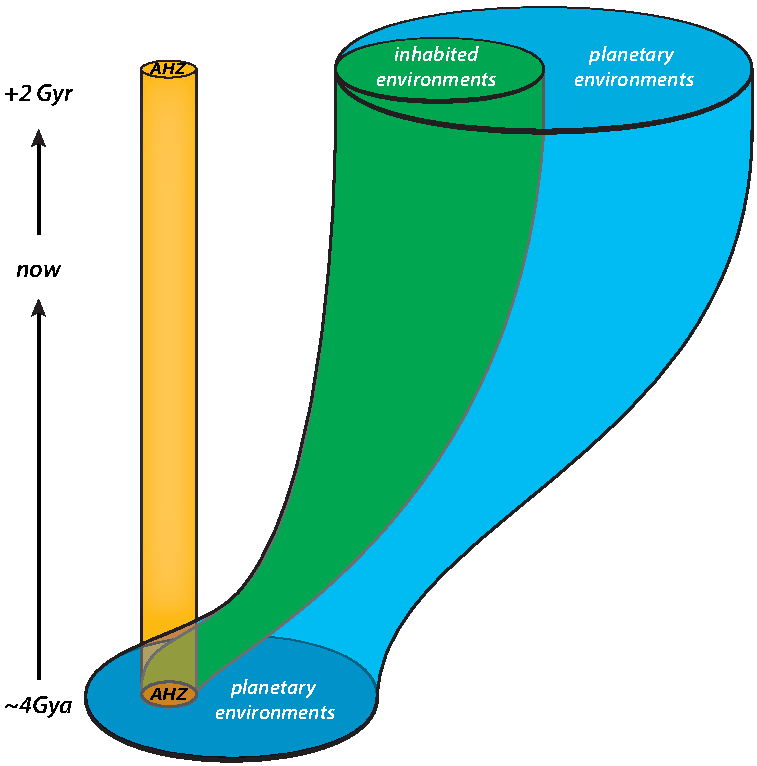
\includegraphics[width=0.6\linewidth]{figures/AHZ.pdf}
	\caption[Abiogenesis Habitable Zone]{The conditions needed for the origin of life are in the Abiogenesis Habitable Zone  or ``AHZ.''
		Inhabited environments (green) are a subset of planetary environments (blue).
		Both of these can change with time.
		The AHZ conditions are probably narrower than the broader conditions to which life can now adapt (``inhabited environments'').
		Through its management of the greenhouse and its partitioning of reductants and oxidants, the activity of life increases the range of inhabited environments \citep{Nisbet2007}.
		Hence, the green cylinder emerges out of the AHZ and gets broader with time.
		More specific reasons for this broadening include (1) the evolution of increasingly efficient catalytic enzymes offering tighter control over reaction rates, 
		(2) the ability of new enzymes to access the energy from different redox pairs providing larger $|\Delta G|$ values \citep{Nealson1999}, and
		(3) the evolution of ecosystems \citep{Smith2015}, global level niche construction, and global biogeochemical feedback cycles (see Section \ref{sec:biofeedbacks}) which we refer to as 
		the ``evolution of Gaian regulation of the biosphere.''
		%Life evolved spores to survive dry conditions, anti-freeze to survive at low temperature and salt pumps to survive at high salinity. 
	}
	\label{fig:AHZ}
\end{figure}

\subsection{Emergence Bottlenecks vs Gaian Bottlenecks}
An emergence bottleneck is illustrated in Figure \ref{fig:EmergenceBottleneck}.
The left panel  shows a hypothetical planet with non-evolving planetary conditions.
The right panel shows a more plausible planet which initially had some habitable regions but, through volatile evolution or other
transient factors, lost its surface water and evolved away from habitable conditions (\eg, a runaway greenhouse or runaway glaciated planet).
Without significant abiotic negative feedback mechanisms, the surface environments of initially wet rocky planets are volatile and change rapidly
without any tendency to maintain the habitability that they may have temporarily possessed as their early unstable surface temperatures transited
through habitable conditions (Figure \ref{fig:GaianHZ} C).
%%%%%%%%%%%%%%%%%%%%%%%%%%%%%%%%%%%%%%%%%%
\begin{figure}[!t]
	\centering
	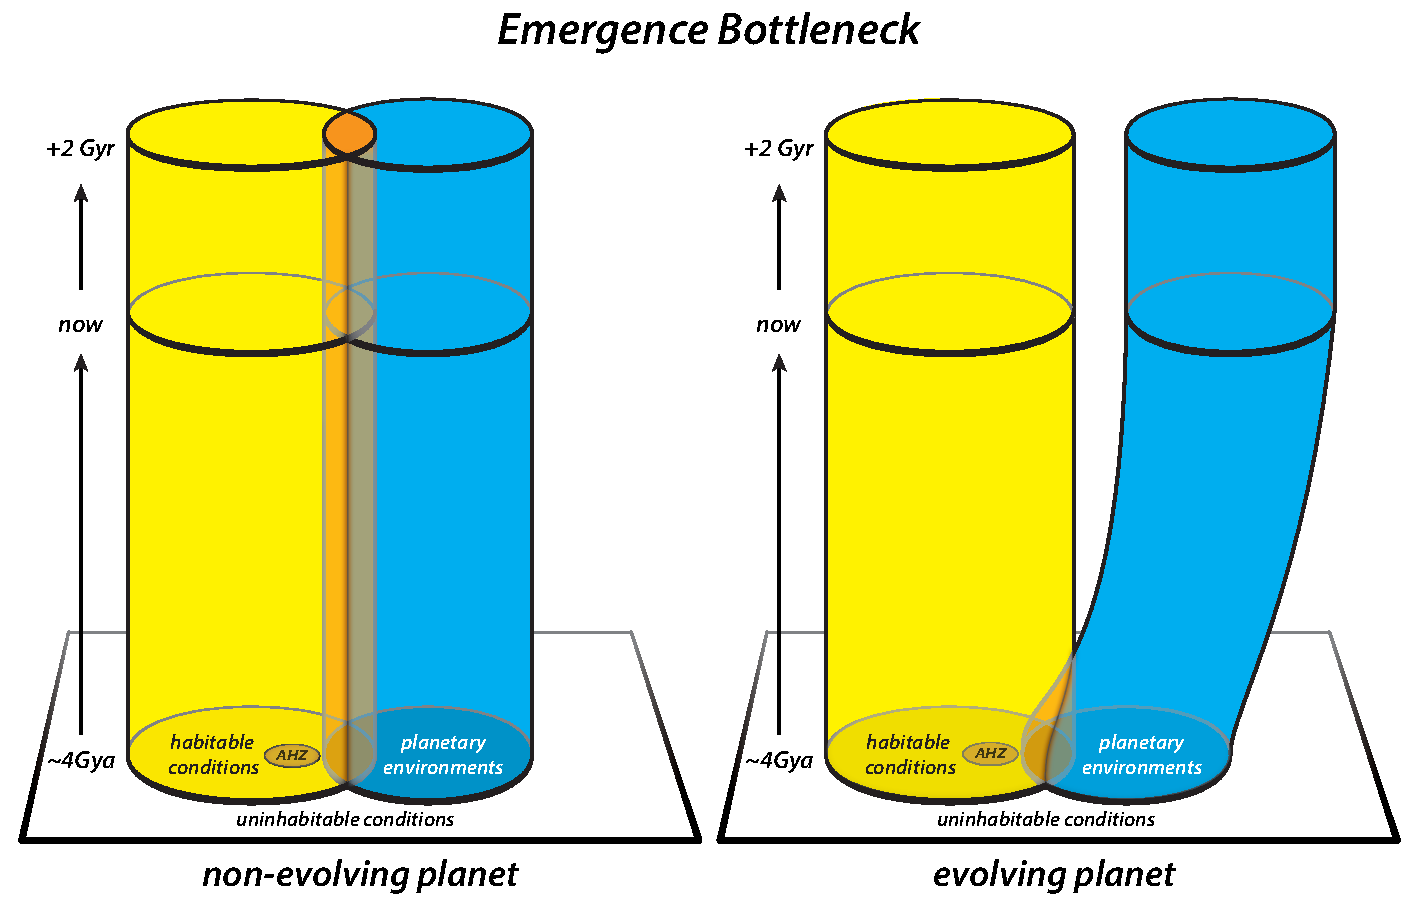
\includegraphics[width=0.9\linewidth]{figures/EmergenceBottleneck.pdf}
	\caption[Emergence Bottleneck]{Emergence Bottleneck: planets on which life does not get started.
		Here, we show habitable conditions (yellow) and planetary environments (blue), from the time of planet formation at the bottom to $\sim$6 billion years later at the top.
		Life will not emerge on either of these planets since their initial planetary environments do not overlap with the Abiogenesis Habitable Zone (AHZ) where life could get started.
		Both of these planets are initially habitable since their environments overlap with habitable conditions. \textit{Left panel:} In this unrealistic, non-evolving model, planetary environments do not change with time. Habitable regions remain uninhabited because life does not get started. 
		Such planets are uninhabited but remain habitable. \textit{Right panel:}  Parts of this evolving planet were habitable, but life does not emerge. The planet undergoes abiotic evolution and moves quickly away from habitability.
		We argue (Section \ref{sec:awayfromhabitability}) that evolution away from habitability is probably the default for initially wet rocky planets.
		We would find such planets to be uninhabited (and if older than $\sim$1 Gyr, uninhabitable) -- consistent with the idea that a planet has to be inhabited to remain habitable.}
	\label{fig:EmergenceBottleneck}
\end{figure}
%%%%%%%%%%%%%%%%%%%%%%%%%%%%%%%%%%%%%%%%%%
If there is no emergence bottleneck (Figure \ref{fig:GaianBottleneck}), typical wet rocky planets have initial conditions compatible with the emergence of life (AHZ). We postulate that almost all initially wet rocky planets on which life emerges (left panel of Figure \ref{fig:GaianBottleneck}) quickly evolve like the abiotic planets  represented in the right panel of Figure \ref{fig:EmergenceBottleneck}. This unregulated evolution of planetary environments away from habitable conditions constrains the duration of life's existence on the planet. We call this early extinction of almost all life that ever emerges the \textit{Gaian bottleneck}. In rare cases (for example on Earth), life will be able to evolve quickly enough to begin to regulate surface volatiles through the modification of abiotic feedbacks (right panel of Figure \ref{fig:GaianBottleneck}). The potentially relevant feedbacks involved in such early Gaian regulation are illustrated in Figure \ref{fig:feedbacks} and discussed in Table~\ref{tab:feedbacks} and Section \ref{sec:biofeedbacks}.
%%%%%%%%%%%%%%%%%%%%%%%%%%%%%%%%%%%%%%%%%%
\begin{figure*}[!t]
	\centering
	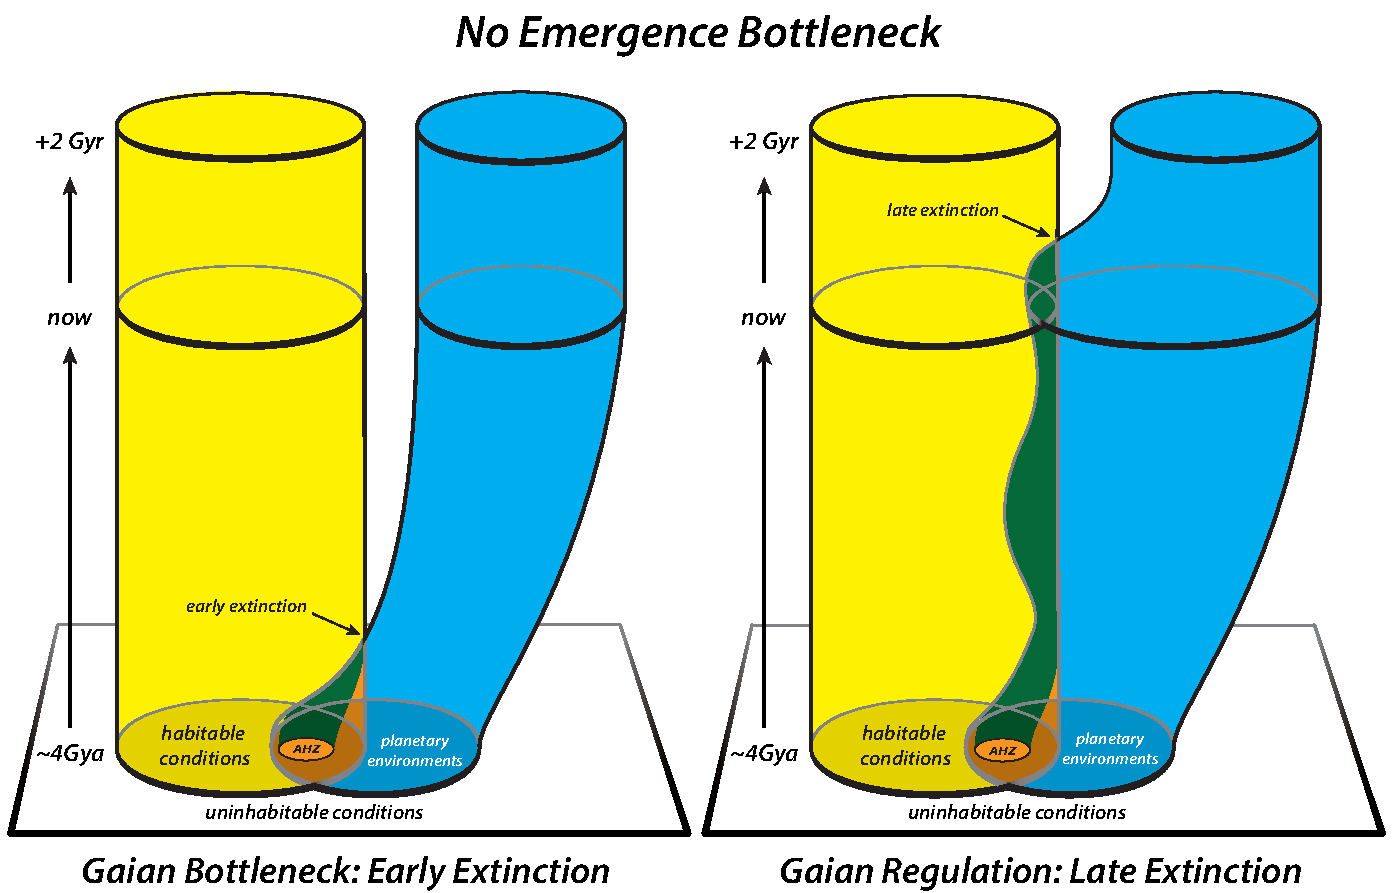
\includegraphics[width=0.9\linewidth]{figures/GaianRegulation.pdf}
	\caption[Gaian Regulation]{The Abiogenesis Habitable Zone may be a very common subset of the environments of rocky planets that are wet during their first billion years.
		As in the left panel of Figure \ref{fig:EmergenceBottleneck}, we assume that these planets are unregulated by any abiotic negative feedbacks and have no tendency to maintain habitability.
		We assume that life gets started on both these planets, so there is no ``emergence bottleneck'' (Section \ref{sec:EmergenceBottleneck}) as there was in
		Figure \ref{fig:EmergenceBottleneck}.
		\textit{Left panel:} Life is unable to evolve rapidly enough to control runaway positive feedbacks.
		Gaian regulation does not emerge fast enough to maintain habitability. 
		Thus, we have a ``Gaian bottleneck.'' We propose that most wet rocky planets are of this kind.
		\textit{Right panel:} In rare cases (as on Earth), Gaian regulation evolves fast enough to make it through the Gaian bottleneck and
		keep at least part of the planet habitable for billions of years. 
		Biospheric regulation maintains the habitability of the planet until $\sim$5 Gyr after formation, at which time, increasing stellar luminosity and loss of water
		cause life to go extinct.
		Extinction happens in both panels but much later in the right panel.
		This figure illustrates our hypothesis that the emergence and rapid extinction of life may be quite common (left) but that the emergence of life, followed by the evolution of Gaian regulation and the long term persistence of life, could be quite rare (right).}
	\label{fig:GaianBottleneck}
\end{figure*}

\section{Early extinction in the first billion years}
\subsection{Bombardment and impact frustration}

During the late phases of Earth's accretion ($\sim$4.5 to $\sim$4.0 Gya), episodes of cold ``Norse ice-hell'' were punctuated by
brief periods of hot inferno with magma oceans \citep{Nisbet2002,Elkins-Tanton2008}. 
Frequent, large, random impacts produced wide-ranging, unstable temperatures.
The largest impacts were so large that any life that did emerge during the transitory habitable periods was probably bombarded into extinction.
These early bombardment-induced extinctions have been called the impact frustration of life \citep{Maher1988,Sleep1989,Sleep2014,Davies2005,Marchi2014}.
The early heavy bombardment of Earth decreased by more than $\sim$13 orders of magnitude during this period (\citet{Bland2005,Koberl2006} 
Figure \ref{fig:GaianHZ} A).
As the rate of planetary accretion slowed, the impact rate and the size of the largest impactors decreased.
Habitable conditions became, at least fleetingly, more available for life \citep{Abramov2009,Abramov2013}. Impact heating may have provided strong selection pressure on early life to evolve into deep environments to survive thermal perturbations \citep{Sleep1989,Nisbet2001,Mat2008}.

We have no reason to believe that these processes are specific to Earth or to our Solar System. The surfaces of Earth-sized rocky planets will undergo an early heavy bombardment that produces severe intermittent temperature pulses. A decreasing bombardment rate is likely to be a generic process that controls the emergence and early persistence of life  on wet rocky planets near the circumstellar habitable zones of host stars throughout the universe. As the bombardment rate decreases, these rocky planets cool down and can harbour, at least temporarily, habitable environments where life can emerge from primordial soups, hydrothermal vents, or any other AHZ candidate. 
Whether life usually persists after this emergence is what we are calling into question. 

We postulate that the combination of heavy bombardment, volatile evolution, and thermal instability almost always conspires to eliminate incipient life before it has a chance to evolve sufficiently to regulate initially abiotic global cycles. We also postulate that exceptionally, life on Earth was able to counter the effects of volatile evolution, thermal instability, and the general abiotic tendency to drift away from habitability. In other words, we argue that the same catastrophic events that life on Earth seems to have overcome, usually lead to extinction. In the first billion years on a wet rocky planet in the universe, impacts and an inability to control surface environments are usually not just frustrating, 
but fatal.
\subsection{Devolatilization of habitable planets}
\label{sec:awayfromhabitability}

Liquid water is not easy to maintain on a planetary surface. The initial inventory and the timescale with which water is lost to space due to a runaway greenhouse, or frozen due to ice-albedo positive feedback, are poorly quantified, but plausible estimates of future trajectories have been made. On Earth, dissociation of water vapor by ultraviolet radiation in the upper atmosphere
is ongoing and will eventually ($\sim$1-2 billion years from now) lead to the loss of water from the bio-shell and the subsequent extinction of life on Earth \citep{Caldeira1992,Franck2000,Lenton2001,Franck2002,vonBloh2005}.


In our Solar System, Venus, Earth, and Mars are usually assumed to have started out in similar conditions: hot from accretion and wet from the impacts of aqueous bodies from beyond the snowline. However, atmospheric evolution of these planets diverged significantly \citep{Kasting1988,Kulikov2007,Driscoll2013}. The simplest interpretation of the D/H ratios of Venus:Mars:Earth:Sun (2000:70:10:1) is that (i) Venus has lost the vast majority of its H$_{2}$O, (ii) Mars lost about $85\%$ of its initial water content and the rest froze into the polar ice-caps and subsurface permafrost \citep{Kurokawa2014,Villanueva2015a} and (iii) Earth was able to keep a larger fraction of its H$_{2}$O (\citet{Pope2012}, Figure \ref{fig:inventory}).

%%%%%%%%%%%%%%%%%%%%%%%%%%%%%%%%%%%%%%%%%%
\begin{figure}[!htbp]
	\centering
	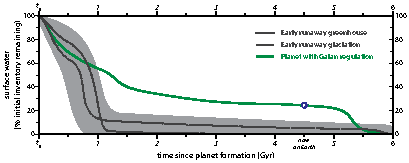
\includegraphics[width=1.0\linewidth]{figures/WaterInventory.pdf}
	\caption[Water loss on initially `wet' rocky planets]{
		Schematic illustration of the water loss caused by impacts and hydrogen escape.
		Hydrogen escape may entirely desiccate a rocky planet within a few billion years \citep{Lovelock2005}. Desiccation is inevitable as the host star luminosity increases, a cold trap is lost and the stratosphere becomes moist \citep{Lenton2001,OMalley-James2015}.}
	\label{fig:inventory}
\end{figure}
%%%%%%%%%%%%%%%%%%%%%%%%%%%%%%%%%%%%%%%%%%%%%%%%%%%%%%

However, the answer to the question ``Why didn't Earth undergo runaway greenhouse like Venus or a runaway glaciation like Mars?'' may have as much, or more, to do with life on Earth than with Earth's distance from the Sun.
The biotic mechanisms of how this preservation has been achieved have been discussed in the context of the Gaia Hypothesis by \citet{Harding2010}.

The early devolatilization of Earth-like planets around M-stars due to an extended pre-main sequence period of high extreme UV flux (above the dissociation energy of water, $\sim$5 eV)  could apply to some extent to Earth-like planets around more massive stars \citep{Luger2015,Tian2015}.

The amount of water (and volatiles in general) deposited or devolatilized during the late accretion phase of rocky planet formation in the universe is highly variable \citep{Raymond2004,Raymond2009} and can produce desert worlds \citep{Abe2011}, ocean worlds \citep{Leger2004}, and probably everything in between. Abiotic volatile evolution will be rapid, stochastic and hostage to the timing, mass, volatile content, and impact parameters of the largest impactors and the runaway feedbacks they could induce.

We argue that abiotic habitable zones are available initially and fleetingly to wet planets within a wide range of orbital radii ($\sim$0.5 to $\sim$2 AU) because of the thermal instability of their surfaces. Wide-ranging unstable temperatures could provide transitory abiotic habitable zones during the first half billion years after formation (\citet{Nisbet2002}, Figure \ref{fig:GaianHZ} B and \ref{fig:GaianHZ} C).

There are two ways to influence the surface temperature of a planet (Figure \ref{fig:feedbacks}): change the albedo (grey loops)  or  change the greenhouse gas content of the atmosphere (blue loops) \citep{Kasting2012}.
The amount and the phases of the volatiles (H$_{2}$O, CO$_{2}$, CH$_{4}$) of rocky planetary atmospheres control both the albedo and greenhouse warming.
Albedo and greenhouse warming, in turn, control the amount and phases of the volatiles. Strong positive feedback cycles (left side of Figure \ref{fig:feedbacks})  may lead to both i) runaway greenhouse (temperatures too hot for
life) with runaway loss of atmosphere (hydrogen loss and thus water loss) or ii) runaway glaciation (lowering the temperature and/or water activity to levels not conducive to life).

%%%%%%%%%%%%
\subsection{Implausibility of early negative feedback cycles}
\label{sec:silicateweathering}
In his original estimate of the continuous habitable zones, \citet{Hart1979} considered runaway greenhouse and runaway glaciation feedback but did not account for the negative feedback of silicate weathering on his models. The resulting continuous habitable zone of 0.95-1.01 AU had such a narrow width that he wrote:
\begin{quotation}
	It appears, therefore, that there are probably fewer planets in our galaxy suitable for the evolution of advanced civilizations than has previously been thought.
\end{quotation}

Such a narrow CHZ could help solve the Fermi paradox \citep[\eg,][Solution 36, p.158]{Webb2002}. More recent work has taken into account a stabilizing negative feedback loop associated with the recycling of CO$_2$ by plate tectonics. \citet{Walker1981} proposed a greenhouse-gas-based negative feedback process employing the carbonate-silicate cycle through the mechanism of silicate weathering. Increasing surface temperatures increases the silicate weathering rate, freeing up more Ca$^{2+}$ and other cations that combine with CO$_2$ (via aqueous bicarbonate HCO$_{3}^{-}$) to produce insoluble carbonates. Thus, when the temperature rises, more atmospheric CO$_2$ is sequestered and temperature decreases (Walker 1985, and the blue negative feedback loop on the right side of Figure \ref{fig:feedbacks}).
This abiotic negative feedback is largely responsible for moving the outer edge of the CHZ from 1.01 AU, as estimated by \citet{Hart1979}, to the more modern, larger values of 1.5-1.7 AU \citep[\eg,][]{Kasting1993a,Kopparapu2013}.

%%%%%%%%%%%%%%%%%%%%%%%%%%%%%%%%%%%%%%%%%%%%%%%%%%%%%%%%%%
\begin{figure*}[!tbp]
	\centering
	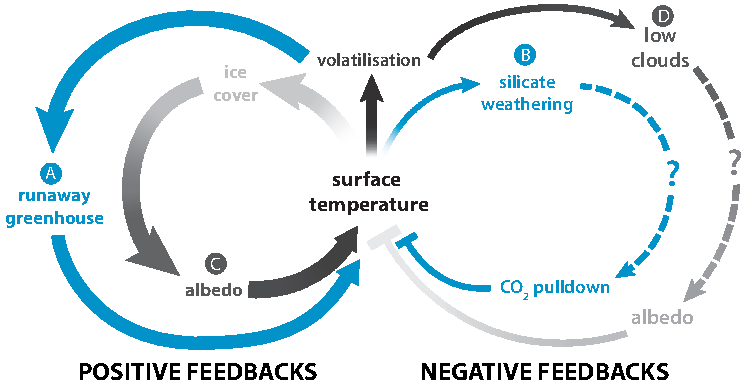
\includegraphics[width=0.9\linewidth]{figures/Feedback.pdf}
	\caption[Early abiotic feedbacks on Earth-like planets]{Early Abiotic Feedbacks.
		During the first billion years after the formation of Earth (or of Earth-like planets), abiotic positive feedbacks (left) can lead to runaway surface temperatures outside the habitable range (both too hot and too cold). These positive feedbacks lead to the loss of liquid water (either from hydrogen escape to space or condensation into ice (Figure \ref{fig:inventory})). Abiotic negative feedbacks (right) have been invoked to stabilize surface temperatures, but they may not be significant in the first billion years, hence the dashed lines
		and the question marks (Section \ref{sec:silicateweathering}).
		As life evolves, it can strengthen or weaken these initially abiotic geochemical feedback loops and turn them into biogeochemical cycles and feedback loops. Evolving life can insert itself into these feedbacks at the points labelled A, B, C and D. (Table \ref{tab:feedbacks} and Section \ref{sec:biofeedbacks}).
	}
	\label{fig:feedbacks}
\end{figure*}
%%%%%%%%%%%%%%%%%%%%%%%%%%%%%%%%%%%%%%%%%%%%%%%

%%%%%%%%%%%%%%%%%%%%%%%%%%%%%%%%%%%%%%%%%%%%%%%%%%%%%%%%%%
\begin{table*}[!ht]
	\centering
	\caption{Abiotic feedback processes active during the first billion years of a wet rocky planet's history and potential biotic enhancements of the feedback cycle.}
	\label{tab:feedbacks}
	\resizebox{1\textwidth}{!}{ 
		\begin{tabular}{l p{6.3cm} l p{7.2cm} }
			%{@{}lll|@{}}
			%\toprule
			Feedback       	& Mechanism	& Feedback Type		& Potential Biological Mediation\\
			\midrule
			greenhouse     	& greenhouse gases \citep{Ingersoll1969,Abe2011} 	 	& positive			& \textbf{A} \citep{Catling2001,Kasting2012,Goldblatt2009,Harding2010}\\
			greenhouse     	& silicate weathering \citep{Walker1981}   & negative?        	& \textbf{B} \citep{Lovelock1982,Schwartzman1989,Catling2001,Rosing2006,Honing2014}\\
			albedo          & ice albedo \citep{Budyko1969,Hoffman1998,Kopp2005}         & positive         	& \textbf{C} \citep{Harding2010,Watson1983}\\
			albedo          & low clouds \citep{Abe2011}          & negative?       	& \textbf{D} \citep{Rosing2010}\\  
			\bottomrule
		\end{tabular}
	}
	
\end{table*}
%%%%%%%%%%%%%%%%%%%%%%%%%%%%%%%%%%%%%%%%%%%%%%%%%%%%%%%%%


Since the temperature-dependent carbonate-silicate cycle provides a negative feedback, it could have been responsible for the long term stabilization of Earth's surface temperature. With a sufficiently high silicate weathering rate, even a lifeless planet could remain habitable. However, since temperature-dependent silicate weathering requires sub-aerial weathering of silicate rocks (either granitic or basaltic), the magnitude of the negative feedback of silicate weathering is roughly proportional to the amount of sub-aerial continental crust. In the first billion years of Earth's history, the fraction of the surface of Earth where sub-aerial erosion would have been possible may have been extremely small \citep{Flament2008,Abbot2012,Dhuime2015}. \citet{Flament2008} modeled the sub-aerial weathering as a function of time and estimated that in the late-Archean ($\sim$2.5 Gya)  2-3\%  of the Earth's surface was sub-aerial continent. The little continental crust present was largely submerged. Thus, it is likely that early in Earth's history, the negative feedback of the carbonate-silicate cycle may have been inoperative or at least significantly less effective than today. This undermines the main negative feedback mechanism proposed to stabilize surface temperature on wet rocky planets for the first billion years or so, when they are most likely to experience runaway greenhouse or runaway glaciation due to high inventories of primordial greenhouse gases, higher bombardment rates, and higher volcanism: hence, the ``?'' associated with this negative feedback loop in Figure \ref{fig:feedbacks} and Table \ref{tab:feedbacks}. Without this abiotic feedback cycle to extend the outer edge of the CHZ, the much narrower Hart-like continuously habitable zone (Figure \ref{fig:GaianHZ} B) becomes more plausible.

%%%%%%%%%%%%%%%%%%%%%%%%%%%%%%%%%%%%%%%%%%
\begin{figure*}[!htbp]
	\centering
	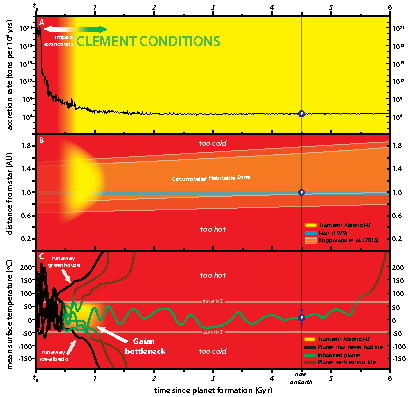
\includegraphics[width=0.9\linewidth]{figures/HZs.pdf}
	\caption[Habitable zones and the Gaian bottleneck]{
Bombardment, habitable zones, and the Gaian bottleneck.
\textbf{A}. Early heavy bombardment precludes life for the first $\sim$0.5 billion years, indicated by red in all three panels.
These impacts produce heat pulses and both deliver and remove volatiles \citep{Elkins-Tanton2011a}. 
Thus, the \textit{amount} of H$_{2}$O at the surface is highly variable during this period.
The \textit{phase} of the H$_{2}$O at the surface is also highly variable during this period because of impact-induced
alternation between greenhouse warming and ice-albedo runaway.
%
\textbf{B}. The width of the circumstellar habitable zone (CHZ) is usually considered to be a function of physics and chemistry, but
is often computed without the largely uncertain influence of clouds, and placed between Venus (0.7 AU) and Mars (1.5 AU). Here the blue region is from the work of \citet{Hart1979}, and the orange regions are based on estimates by \citet{Kopparapu2013} for the conservative (light orange) and optimistic (dark orange) limits. Life plays no role in these computations. The $\sim$30\% increase in the luminosity of the Sun since its formation is responsible for the outward migration of the traditional CHZ and some of the narrowness of Hart's continuously habitable zone.
The yellow zone in B represents our speculative version of a short-lived abiotic habitable zone at the tail end of the impact-induced
thermal instabilities shown in the first billion years of panel \textbf{C}.
The width of the abiotic habitable zone begins with a fairly wide range of semi-major axes, but lasts only from $\sim$0.5 to $\sim$1 Gyr
and then shrinks to zero.
After $\sim$1 Gyr, rapid impact-induced thermal excursions diminish and surface temperatures drift away and runaway from habitability.
Planets become devolatized because of the runaway greenhouse effect (top of panel C), 
and because liquid water condenses out into ice due to the runaway ice-albedo effect (bottom of panel C), with no abiotically stable zone between them.
The early evolution of Gaian regulation may be the main feature responsible for maintaining the surface temperature of Earth within a habitable range for the past $\sim$4 billion years \citep{Lovelock2000}.
	}
	\label{fig:GaianHZ}
\end{figure*}
%%%%%%%%%%%%%%%%%%%%%%%%%%%%%%%%%%%%%%%%%%%%%%%%%%%%%% 

The other abiotic negative feedback on surface temperature shown in Figure \ref{fig:feedbacks} is associated with low clouds:
higher temperatures  $\rightarrow$ more volatilization $\rightarrow$ more low altitude clouds  $\rightarrow$ higher albedo  $\rightarrow$ lower temperatures. Low clouds increase albedo and decrease surface temperatures more than they contribute towards raising the surface temperature because of the greenhouse effect associated with clouds \citep{Abe2011}. This is problematic because increasing volatilization produces both i) more low altitude clouds (which could cool Earth due to their higher albedo), and more high altitude clouds, which could have a stronger greenhouse effect than albedo effect and thus increase surfaces temperatures \citep{Goldblatt2011,Leconte2013}. For this reason, the effects of clouds are often considered the biggest source of uncertainty in global climate models and thus the ``?'' associated with this cycle in Figure \ref{fig:feedbacks} and Table \ref{tab:feedbacks}.

While it may be possible to vary albedo and greenhouse gases within some plausible range and construct a wide CHZ, without negative feedback, there is no justification for tuning these abiotic variables to maintain habitability. We postulate that the abiotic stabilizing feedbacks (two cycles on the right side of Figure \ref{fig:feedbacks}) were probably negligible
on early Earth. In their absence, it is hard to understand how habitability would have been maintained. Driver-less cars don't stay on roads. Without significant abiotic stabilization, we propose that the most plausible default becomes the abiotic tendency to evolve away from habitability shown in Figure \ref{fig:AHZ}
and Figure \ref{fig:GaianHZ} C.

Just because Earth is at 1 AU and has been inhabited for $\sim$4  billion years does not mean that there is a physics-based, biology-independent, computable continuous habitable zone. With thermal instability and increasing stellar luminosity, it is not clear that a physics-based continuously habitable zone even exists. There may be no range of orbital distances (or any region of multi-dimensional abiotic parameter space) for which the surface environments of initially wet rocky planets have sufficiently strong abiotic negative feedback to maintain habitability. If this is the case, purely abiotic computations of a continuously habitable zone may be misleading, and Gaian regulation becomes a plausible explanation for the continuously inhabited HZ in which we find ourselves.

%%%%%%%%%%%%%%%%%%%%%%%%%%%%%%%%

\section{The need for Gaia}
\label{sec:biofeedbacks}

It is usually assumed that the CHZ is determined by abiotic physical parameters: stellar mass and luminosity, planetary mass and 
atmospheric greenhouse gas composition, surface albedo, and sometimes clouds. 
More recently planetary spin, orbital eccentricity, obliquity, and initial water content have been added to the list of physical parameters \citep[\eg,][]{Gonzalez2005,Gaidos2005,Lammer2009,Gudel2014b,Shields2015}. %Armstrong et al 2014 
Here, we argue that these abiotic parameters can fleetingly enable the emergence of life but cannot maintain habitable surface conditions with liquid water.
As the early heavy bombardment subsides, strong selection pressure on life begins to regulate, control, and even dominate the mechanisms that 
create or maintain the temperatures and pressures at the surface of a planet that allow liquid water. If so, then biology (rather than physics or chemistry) can play the most important role in maintaining habitability.

In addition to the abiotic environmental changes (due to bombardment and devolatilization), there could be a long struggle that starts early between life and an environment that does not, abiotically, stay habitable. Feedback between life and environment may play the dominant role in maintaining the habitability of the few rocky planets in which life has been able to evolve Gaian regulation quickly.

If life gets started on a planet, there are many potential ways in which life can regulate the mechanisms that create or maintain 
the temperatures and pressures needed for liquid water \citep{Schneider1991,Schneider2004,Harding2010}. Gaia researchers propose that life on Earth evolved to become integrated into previously abiotic feedback systems that can modify or regulate surface temperature and the hydrological cycle \citep[\eg,][]{Lenton1998,Nisbet2012}. Life can evolve to enhance and regulate the feedback loops  (biological mediation processes A-D in Figure \ref{fig:feedbacks} and Table \ref{tab:feedbacks}).
Biologically mediated feedback loops are stabilizing or Gaian \citep{Ricklefs2000}. For habitability to be maintained, life could down-regulate the positive runaway feedback loops and enhance the negative feedback loops. On Earth, life began to modulate the greenhouse gases composition of the atmosphere as soon as life became widespread \citep{Nisbet2002,Nisbet2012,Nisbet2014,Johnson2015}.

The use of the Gaia hypothesis in ecology was reviewed by \citet{Free2007}. They argued (in agreement with \citet{Dawkins1982}) that selection for global stability is implausible.
However, they defined a Probable Homeostatic Gaia model: a planet ``with appropriate starting conditions for life will probably generate a biosphere the lifespan of which will be extended, rather than reduced, by life-environment feedback.'' In their Probable Homeostatic Gaia model, a ``network of life-environment interactions, largely dependent on the by-product effects of evolved traits, leads to global stability.''
This biology-based global stability is what we call Gaian regulation.  We are invoking its rapid evolution to stabilize the early volatile and thermal
instabilities of wet rocky planets.
%See Schneider \& Boston 1991 and Schneider et al 2004 for more discussion.
% cite O'Malley James and Cocknell 2015?

If Gaian regulation plays the dominant role in maintaining liquid water at the surface \citep{Harding2010}, then the width of the CHZ would depend more on 
the quirks of biological evolution than on the more deterministic physics and chemistry that can be more easily modeled. For most rocky planets in the CHZ to remain habitable, they may have to be inhabited:
``habitability depends on inhabitance and the width of the habitable zone is difficult to characterize'' \citep{Goldblatt2015}.


In Gaian literature, it is usually proposed that  Earth became a Gaian planet in the Proterozoic ($\sim$2.5 Gya) and has been one ever since \citep[p.45]{Harding2010}. We are proposing that the onset of Gaian regulation could have occurred more than a billion years earlier, for example, through the production, consumption, and regulation of greenhouse active gases such as H$_{2}$, CO$_{2}$, and CH$_{4}$. If there is a biotic solution for the faint early Sun paradox \citep{Sagan1972,Sagan1997,Feulner2012} based on higher concentrations of CO$_2$, on biotic methanogenesis, or on biotic albedo regulation, then this solution would necessarily have evolved quickly during the transient abiotic HZ (yellow regions in Figure \ref{fig:GaianHZ} B and C) \citep{Walker1985,Pavlov2003,Haqq-Misra2008,Rosing2010}.

\section{Evaluating the Gaian Bottleneck Hypothesis}

%%%%%%%%%%%%%%%%%%%%%%%%%%%%%%%%%%%%%%%%%%%%%%%%%%%%%%%%%%
\begin{figure*}[!b]
	\centering
	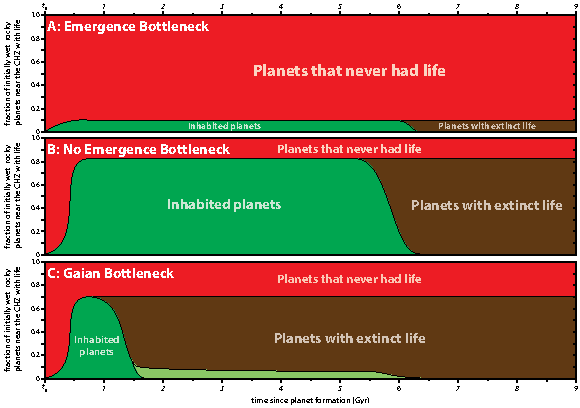
\includegraphics[width=0.9\linewidth]{figures/Summary.pdf}
	\caption[Different bottleneck scenarios]{Different bottleneck scenarios and their fossil predictions.
		\textbf{A}. Emergence Bottleneck: Life rarely emerges even on wet rocky planets. Few planets will have life or even fossils of extinct life.
		On the few planets where life does emerge, it persists for billions of years. 
		\textbf{B}. No Emergence Bottleneck.  Life emerges with high probability and usually persists for billions of years. Thus, life will be abundant on planets throughout the universe. There will be many planets where life persisted for billions of years and then went extinct. On the oldest uninhabited planets, fossils of complex  life will be abundant.
		\textbf{C}. Gaian Bottleneck. Life emerges with some probability (possibly quite high), but it goes extinct within a billion years (green). Alternatively, some small fraction of inhabited planets successfully pass through the Gaian bottleneck (light green). The Gaian bottleneck model predicts that the vast majority of the fossils in the universe will be from extinct microbial life.}
	\label{fig:summary}
\end{figure*}
%%%%%%%%%%%%%%%%%%%%%%%%%%%%%%%%%%%%%%%%%%%%%%%

After the early heavy bombardment, life emerges with some probability on initially wet rocky planets in the CHZ.
However, due to large impacts and unstable abiotic volatile evolution with no
tendency to maintain habitability, almost all life goes extinct early -- with the rare exceptions of life
that has undergone unusually rapid evolution and obtained some level of Gaian regulation. The most significant predictions of this Gaian bottleneck model can be seen in Figure \ref{fig:summary} by comparing panels A and B, with C.
In panels A and B, wherever life emerges, it persists for billions of years. Thus, it has time to evolve complex and perhaps multicellular forms. In panel C, which illustrates the Gaian bottleneck model, almost all emerging life goes extinct rapidly and therefore, does not have time to evolve into more complex forms.
However, even planets with Gaian regulation will not be able to counter indefinitely the increasing luminosity due to stellar evolution  \citep{Caldeira1992,Franck2000,Lenton2001,Franck2002,vonBloh2005}. Hence, the extinction at $\sim$6 Gyr in all 3 panels.

If we are able to find well-preserved, $\sim$3.8 to $\sim$4.3 billion year old rocks on Venus or Mars, then we may be able to identify
isotopic anomalies produced by biotic actions, in a way analogous to how $^{12}$C/$^{13}$C ratios are used to infer the existence of the earliest life in Isua, Greenland \citep{Ohtomo2014}. Whether it evolved independently of life on Earth will be difficult to determine. If we find evidence of extant life on Mars or Venus that had an origin independent of Earth life, then this would be evidence against both the Gaian bottleneck hypothesis and the emergence bottleneck.

The surface temperature and existence of liquid water at, or near, the surface could be predominantly due to Gaian regulation rather than abiotic negative  feedback. Liquid water on the surface of the planet (particularly old planets) would then not just be a prerequisite for life but a biosignature \citep{Gorshkov2004}. Existence of liquid water on the surface of a planet may be a better biosignature than oxygen \citep{Luger2015}. Thus, the measurement of exoplanet surface temperatures compatible with liquid water could be an important part of future search for extra-terrestrial life. Remote detection of atmospheric chemical equilibrium may soon develop into a mature science of remote bio-detection \citep[\eg,][]{Lovelock1975,Krissansen-Totton2016}. The Gaian bottleneck model predicts that the vast majority of the atmospheres of old terrestrial planets in the traditional abiotic CHZ of their host stars will be in chemical equilibrium because they are uninhabited. Hence, atmospheres in chemical disequilibrium will be rare except for young (t $\lesssim$ 2 Gyr) terrestrial planets.

In a critique of Gaian logic, \citet[p.236]{Dawkins1982} wrote:
\begin{quotation}
	For the analogy [of the Earth as an organism] to apply strictly, there would have to have been a set of rival Gaias, presumably on different planets. Biospheres which did not develop
	efficient homeostatic regulation of their planetary atmospheres tended to go extinct. The
	Universe would have to be full of dead planets whose homeostatic regulation systems had failed,
	with, dotted around, a handful of successful, well-regulated planets of which the Earth is one''.
\end{quotation}

What Dawkins describes here is also a prediction of the Gaian bottleneck hypothesis. The Gaian bottleneck model parallels evolution on Earth in that the vast majority ($\sim$99.9\%) of species that have ever lived are now extinct; the vast majority of planetary life has gone extinct.

In the far future, we may be able to find evidence for biogenic isotopic anomalies on the initially wet rocky planets around most stars. Since life does not persist for long in the Gaian bottleneck model, it predicts a universe filled with isotopic or microscopic fossils
from the kind of life that can evolve in $\sim$1 Gyr, not the fossils of larger multicellular eukaryotes or anything else that would take several billion years to evolve.

\citet{Cockell2014} divided all environments in the Universe into three types: (1) uninhabitable, (2) uninhabited habitats or (3) inhabited habitats \citep{Cockell2011,Zuluaga2014}. A prediction of the Gaian bottleneck (persistence-is-hard) model is that (2) and (3) will be rare. This is unfortunate for future colonization efforts since uninhabited, but habitable, planets are the most ethically appealing places -- autochthonous life would not have to be displaced.

Our search for life beyond Earth may be thwarted by the short time-scales over which planets may remain inhabited. If it takes several billion years to develop radio telescopes, then the Gaian bottleneck ensures that the vast majority of life in the universe is either young and microbial, or extinct. Therefore, the Gaian bottleneck model is consistent with current SETI results and can help resolve the Fermi paradox, although it is not one of the solutions to the paradox listed by \citet{Webb2002}.
%%%%%%%%%%%%%%%%%%%%%%%%%%%%%%%%%%%%%%%%

	
\clearpage
\section{What could be wrong with our argument?}
\begin{enumerate}
	\item Gaian regulation is a controversial idea.  It is usually invoked to explain the long-term stability of the surface temperature of Earth, starting in the Proterozoic ($\sim$2.5 Gya). So invoking early, pre-Proterozoic Gaia is even more controversial.
	
	\item If estimates of sub-aerial continental crust \citep[\eg, by][]{Flament2008} are significantly too low and there was abundant sub-aerial crust earlier than  
	$\sim$3.8 Gya \citep[\eg,][]{VanKranendonk2010}, then abiotic negative feedback based on the
	carbonate-silicate cycle could have stabilized surface temperatures very early in Earth's history, without Gaian regulation. If early continent formation
	is a common feature of rocky planets, then invoking Gaian regulation may be unnecessary to explain Earth's early thermal stability.
	
	\item We are arguing that:
	\begin{enumerate}
		\item Gaian regulation evolved on Earth.
		\item The evolution of Gaian regulation is not common.
	\end{enumerate}
	This could seem paradoxical, because to justify (a), we have presented arguments making the emergence of Gaian regulation plausible. 
	These same arguments could suggest that Gaian regulation would be common. However, there is a large class of phenomena that did happen on Earth, that are uncommon or non-existent elsewhere.
	We can trace the evolution of these phenomena and explain how they evolved on Earth, but these explanations cannot be generalized.
	For example, the evolution of the English language can be traced and understood and made plausible, but this plausibility cannot be turned 
	into a generic argument for the evolution of English on other planets. 
	Human-like intelligence may be another member of this class \citep{Lineweaver2008}. We are suggesting that the evolution of a kind of life that can quickly and effectively regulate the volatiles on the surface of the planet on which it finds itself, may be a quirky product of the biological evolution of life on early Earth.
	
	\item Why should Gaian regulation be rare? \citet{Franck2002,Franck2001} concluded that there are $\sim$500,000 ``sister Gaias'' in the Milky Way galaxy but then listed a number of physical factors \citep[\eg, those discussed by][]{Ward2000} that could reduce this estimate.
	
	\item It could be that early heavy impacts almost always extinguish life and don't need any help from subsequent volatile evolution away from habitability. In which case, Gaian regulation would have nothing to do with life's early or late extinction. Evidence for this would be an anomalously low impact rate on Earth (compared to the early impact rates on other wet rocky planets). If this were the case, there would be no tendency for life to evolve and regulate its environment. In this context, \citet{Tyrrell2013} suggested that ``Lucky Gaia'' as described by \citet{Free2007}, and the anthropic principle provide a better explanation for the continued habitability of Earth than ``Probable Gaia,'' which we assume here.
	
	If the probability of the emergence and persistence of life on wet rocky planets were infinitesimally small and there were only one life-harboring planet in the Universe, we would, of necessity, find ourselves on that planet. Therefore, our mere existence cannot be used to infer the probability of life elsewhere. Additionally, invoking a scenario in which persistent life on Earth is exceptional compared to other planets (as we do here) cannot be criticized with an argument such as: if Gaian regulation is rare, then we shouldn't be here. Self-selection overcomes this critique. 

	\item One argument against early Gaian regulation is that the unit of biological selection starts small and moves to larger groups as in the chronological sequence: genes, chromosomes, single cells, colonies of cells (bacterial mats), multicellular organisms, colonies of multicellular organisms (superorganisms), ecosystems of various sizes (which produce Gaian regulation only when they are widespread). In this sequence, the evolution of Gaian regulation happens last. However, among the earliest life forms we know of, stromatolites were already ecosystems of bacterial mats \citep{Walter1992}.
	
	\item The universe does not seem to be teeming with life.
	This could be an observational selection effect: it is teeming with life but we just haven't been able to detect it yet. Even in the future when the remote detection of biosignatures is possible, it will be difficult to detect subsurface life \citep{Boston1992,Gaidos1999,Jones2011,McMahon2013} that does not interact with the planet's atmosphere and is completely sustained by free energy based on geochemical disequilibrium.
	This would undermine some of the motivation for the Gaian bottleneck model but not the other arguments presented here.
\end{enumerate}


\section{Conclusion}
We are proposing a potentially universal sequence of events on initially wet rocky planets that can be summarized thusly:
\begin{itemize}
	\item[]\textbf{First $\sim$0.5 Gyr:} Hot, high bombardment, uninhabitable.
	\item[]\textbf{$\sim$0.5 to $\sim$1.0 Gyr:} Cooler, reduced bombardment, continuous volatile loss.
	\item[]\textbf{$\sim$0.5 to $\sim$1.0 Gyr:} Emergence of life in an environment with a tendency to evolve away from habitability
	\item[]\textbf{$\sim$1.0 to $\sim$1.5 Gyr:} Inability to maintain habitability, followed by extinction.
	As a rare alternative, this period would experience the rapid evolution of Gaian regulation and the maintenance of habitability, followed by the persistence of life for several billion more years. 
\end{itemize}
Between the early heat pulses, freezing, volatile content variation, and runaway positive feedbacks, maintaining life on an initially wet rocky planet in the habitable zone may be like trying to ride a wild bull. Most life falls off.  Life may be rare in the universe, not because it is difficult to get started, but because habitable environments are difficult to maintain during the first billion years.

In the book \textit{Vital Dust}, \citet{DeDuve1995} presented the case that water and energy are common and abiogenesis may be a cosmic imperative. The most important constraint on the existence of life in the universe may be whether life, after emerging and evolving into a biosphere, can evolve global mechanisms 
rapidly enough to mediate the positive and negative feedbacks of abiotic atmospheric evolution. We hypothesize that the early evolution of biologically mediated negative feedback processes, or Gaian regulation as proposed by \citet{Lovelock1974}, may be necessary to maintain habitability because of the strength, rapidity, and universality of abiotic positive feedbacks on the surfaces of rocky planets in traditional CHZs.

We argue that the habitable surface environments of rocky planets usually become uninhabitable due to abiotic runaway positive feedback mechanisms involving surface temperature, albedo, and the loss of atmospheric volatiles. Because of the strength, rapidity, and universality of abiotic positive feedbacks in the atmospheres of rocky planets in traditional CHZs, biotic negative feedback or Gaian regulation may be necessary to maintain habitability.

The evolution of biospheric regulation of surface volatiles, temperature, and albedo can become a Gaian bottleneck to the persistence of life. This Gaian bottleneck may be a better explanation for the non-prevalence of life than the traditional emergence bottleneck paradigm. 